\documentclass[border=10pt]{standalone}

\usepackage{tikz}
\usepackage{tikzsymbols}
\usetikzlibrary{calc,patterns,shapes.geometric}

\def\centerarc[#1](#2)(#3:#4:#5){\draw[#1] ($(#2)+({#5*cos(#3)},{#5*sin(#3)})$) arc (#3:#4:#5);}

\begin{document}
	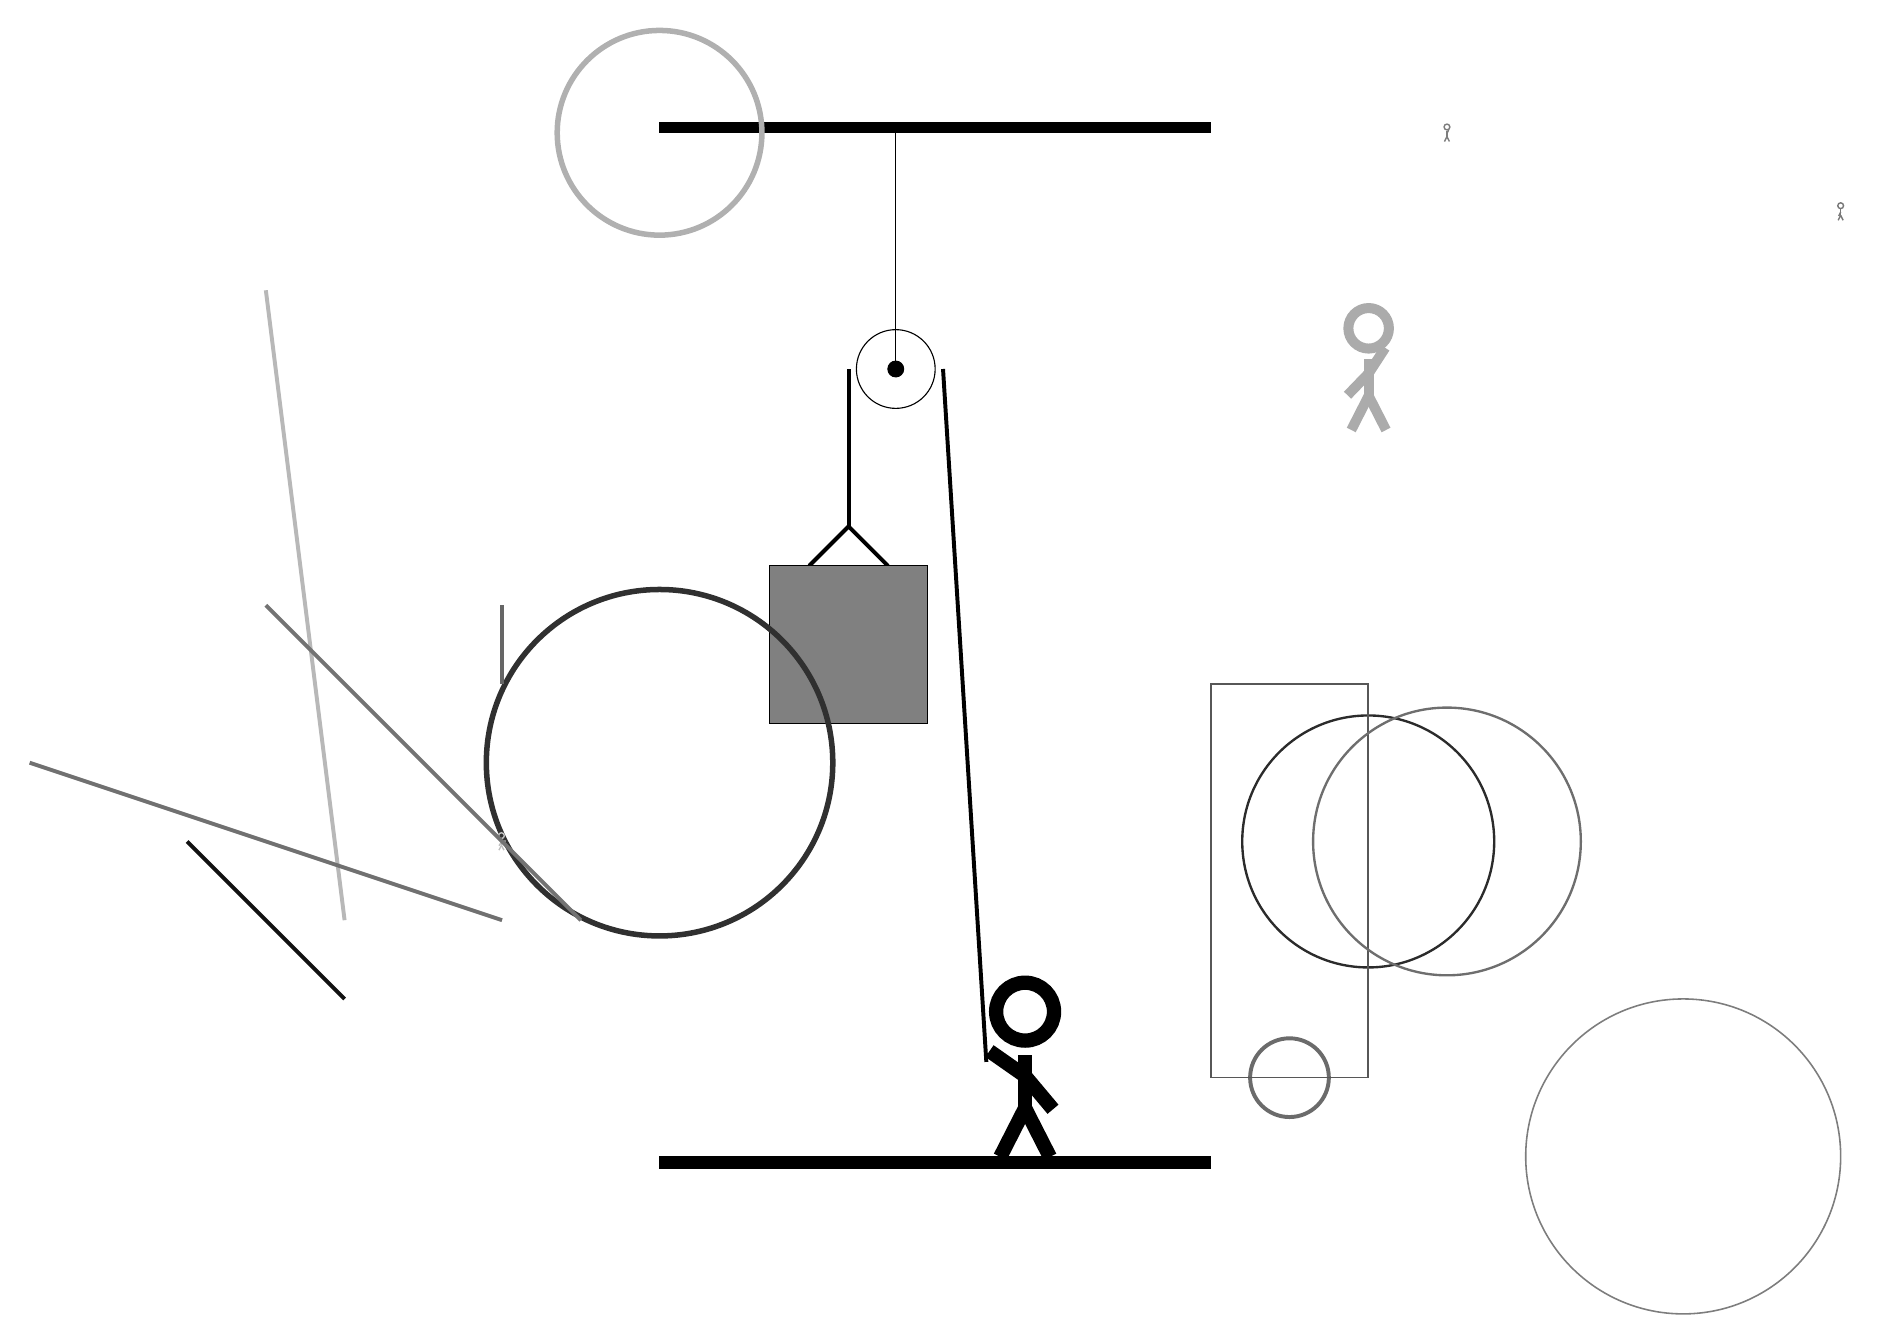
\begin{tikzpicture}
		%%%%% START %%%%%
		
		\draw[fill=black] (-2, 10) rectangle (5, 10.125);
		
		\draw (1, 7) circle (0.5);
		\draw[fill=black] (1, 7) circle (0.1);
		\draw (1, 10) -- (1, 7);
		
		\draw[line width=0.5mm] (-0.1, 4.5) -- (0.4, 5.0) -- (0.9, 4.5);
		\draw[fill=black!50] (-0.6, 4.5) rectangle (1.4, 2.5);
		
		\draw[line width=0.5mm] (0.4, 7) -- (0.4, 5.0);
		\centerarc[line width=0.5mm](1, 7)(0:180:0.6);
		\draw[line width=0.5mm](1.6, 7) -- (2.15, -1.8);
		
		\node at (2.6, -1.9) {\Strichmaxerl[10][-35][-50]};
		
		\node[line width=0.7mm, color=black!33] at (7, 7) {\Strichmaxerl[7][46][57]};
		
		\node[line width=0.6mm, color=black!51] at (8, 10) {\Strichmaxerl[1][89][65]};
		\draw [line width=0.7mm, color=black!81](-2, 2) circle (2.2);
		\node[line width=0.2mm, color=black!53] at (13, 9) {\Strichmaxerl[1][64][90]};
		\draw [line width=0.2mm, color=black!51](11, -3) circle (2.0);
		\draw [line width=0.7mm, color=black!31](-2, 10) circle (1.3);
		\draw [line width=0.3mm, color=black!83](7, 1) circle (1.6);
		\draw [line width=0.5mm, color=black!58](6, -2) circle (0.5);
		\draw[line width=0.5mm, color=black!93](-6, -1) -- (-8, 1);
		
		\node[line width=0.2mm, color=black!25] at (-4, 1) {\Strichmaxerl[1][56][16]};
		\draw[line width=0.5mm, color=black!28](-6, 0) -- (-7, 8);
		
		\draw[line width=0.2mm, color=black!66] (7, -2) rectangle (5, 3);
		\draw[line width=0.5mm, color=black!60](-4, 4) -- (-4, 3);
		\draw[line width=0.5mm, color=black!55](-7, 4) -- (-3, 0);
		\draw [line width=0.3mm, color=black!57](8, 1) circle (1.7);
		\draw[line width=0.5mm, color=black!56](-4, 0) -- (-10, 2);
		
		
		\draw[fill=black] (-2, -3) rectangle (5, -3.15);
		
		%%%%% END %%%%%
	\end{tikzpicture}
\end{document}